\documentclass[conf]{new-aiaa}
%\documentclass[journal]{new-aiaa} for journal papers
\usepackage[utf8]{inputenc}

\usepackage{graphicx}
\usepackage{amsmath}
\usepackage[version=4]{mhchem}
\usepackage{listings}
\usepackage{color}
\usepackage{siunitx}
\usepackage{longtable,tabularx}
\usepackage{subcaption}
\usepackage{cleveref}
\usepackage{appendix}
\setlength\LTleft{0pt}

\title{Simulating 2D-Convection and Diffusion equation.\\}

\author{Ranjithkumar B}
\affil{SC22M008, M.Tech. Aerospace - Aerodynamics and Flight Mechanics}


\definecolor{mygreen}{rgb}{0,0.6,0}
\definecolor{mygray}{rgb}{0.5,0.5,0.5}
\definecolor{mymauve}{rgb}{0.58,0,0.82}

\lstset{
  backgroundcolor=\color{white},   % choose the background color; you must add \usepackage{color} or \usepackage{xcolor}; should come as last argument
  basicstyle=\footnotesize,        % the size of the fonts that are used for the code
  breakatwhitespace=false,         % sets if automatic breaks should only happen at whitespace
  breaklines=true,                 % sets automatic line breaking
  captionpos=b,                    % sets the caption-position to bottom
  commentstyle=\color{mygreen},    % comment style
  deletekeywords={...},            % if you want to delete keywords from the given language
  escapeinside={\%*}{*)},          % if you want to add LaTeX within your code
  extendedchars=true,              % lets you use non-ASCII characters; for 8-bits encodings only, does not work with UTF-8
  firstnumber=0001,                % start line enumeration with line 1000
  frame=single,                    % adds a frame around the code
  keepspaces=true,                 % keeps spaces in text, useful for keeping indentation of code (possibly needs columns=flexible)
  keywordstyle=\color{blue},       % keyword style
  language=FORTRAN,                % the language of the code
  morekeywords={*,...},            % if you want to add more keywords to the set
  numbers=left,                    % where to put the line-numbers; possible values are (none, left, right)
  numbersep=5pt,                   % how far the line-numbers are from the code
  numberstyle=\tiny\color{mygray}, % the style that is used for the line-numbers
  rulecolor=\color{black},         % if not set, the frame-color may be changed on line-breaks within not-black text (e.g. comments (green here))
  showspaces=false,                % show spaces everywhere adding particular underscores; it overrides 'showstringspaces'
  showstringspaces=false,          % underline spaces within strings only
  showtabs=false,                  % show tabs within strings adding particular underscores
  stepnumber=2,                    % the step between two line-numbers. If it's 1, each line will be numbered
  stringstyle=\color{mymauve},     % string literal style
  tabsize=2,                       % sets default tabsize to 2 spaces
  % title=\lstname                   % show the filename of files included with \lstinputlisting; also try caption instead of title
}

\begin{document}

\maketitle

%\section{Nomenclature}
%
%{\renewcommand\arraystretch{1.0}
%	\noindent\begin{longtable*}{@{}l @{\quad=\quad} l@{}}
%		$M$  & Free stream Mach number \\
%		$P$ &    Static pressure \\
%		$P_0$& Toatal pressure \\
%		$\gamma$ & Specific heat coefficient\\
%		$\theta$ & Flow turn angle \\
%		$ \beta $ & Wave angle \\
%		$ M_2$ & Downstream Mach Number\\
%		$ C_p$ & Coefficient of pressure \\
%		$\nu(M) $ & Prandt- Meyer Function
%\end{longtable*}}

% \begin{abstract}
%     This document contains the list of questions along with answers
%     given as tutorial - 01.
% \end{abstract}

\section{Problem Definition}
\begin{enumerate}
	\item 2D linear convection problem using the FTBS method, forward time difference, backward space difference.
	\item 2D linear diffusion with FD in time and CD in space
\end{enumerate}
\subsection{Boundary condition}
\par x=0 and x=2, y=0 and y=2\\
\begin{center}
	\begin{tabular}{c | c | m{2em}}
		t & n & u(x,y,t) v(x,y,t) \\
		\hline
		0$\leq$t$\leq$0.5 & 0$\leq$n$\leq$50 & 1\\
	\end{tabular}
\end{center}
\subsection{Initial condition}
\par t = 0\\
\begin{center}
	\begin{tabular}{c | c | c | c | m{2em}}
		x & i & y & j & u(x,y,t) v(x,y,t) \\
		\hline
		0 & 0 & 0 & 0 & 1 \\
		\hline
		0$\le$x$\leq$0.5 & 0$\le$i$\leq$5 & 0$\le$y$\leq$0.5 & 0$\le$j$\leq$5 & 1\\
		\hline
		0.5$\le$x$\leq$1 & 5$\le$i$\leq$10 & 0.5$\le$y$\leq$1 & 5$\le$j$\leq$10 & 2\\
		\hline
		1$\le$x$\leq$2 & 10$\le$i$\leq$20 & 1$\le$y$\leq$2 & 10$\le$j$\leq$20 & 1\\
		\hline
		2 & 20 & 2 & 20 & 1 \\
	\end{tabular}
\end{center}


\section{Governing Equations}
\par Two dimentional linear convective equations\Cref{linear_conv_01,linear_conv_02}\\
\begin{align}
	\frac{\partial u}{\partial t}+c \frac{\partial u}{\partial x} +c \frac{\partial u}{\partial y} & = 0 \label{linear_conv_01} \\
	\frac{\partial v}{\partial t}+c \frac{\partial v}{\partial x} +c \frac{\partial v}{\partial y} & = 0 \label{linear_conv_02}
\end{align}
\par Two dimentional linear diffusion equations\Cref{linear_diff_01,linear_diff_02}\\
\begin{align}
	\frac{\partial u}{\partial t} & = \nu \left(\frac{\partial^2 u}{\partial x^2} + \frac{\partial^2 u}{\partial y^2} \right) \label{linear_diff_01} \\
	\frac{\partial v}{\partial t} & = \nu \left(\frac{\partial^2 v}{\partial x^2} + \frac{\partial^2 v}{\partial y^2} \right) \label{linear_diff_02}
\end{align}

\section{Numerical calculation}
\par The numerical scheme is used here is the Forward diffrencing in time and Backward diifrencing in space (FTBS) in linear convection and Forward time and cntrakl diffrencing in space in linear diffusion in u component is metioned in \Cref{FTBS_01,FTBS_02,FTCS_01,FTCS_02} \\
\begin{align}
	\frac{u_i^{n+1}-u_i^n}{\Delta t} & =  -c \left( \frac{u_i^n-u_{i-1}^n}{\Delta x} + c\frac{u_i^n-u_{i-1}^n}{\Delta y} \right) \label{FTBS_01} \\
	\frac{v_i^{n+1}-v_i^n}{\Delta t} & =  -c \left( \frac{v_i^n-v_{i-1}^n}{\Delta x} + c\frac{v_i^n-v_{i-1}^n}{\Delta y} \right) \label{FTBS_02} \\
	\frac{u_i^{n+1}-u_i^n}{\Delta t} & = \nu \left( \frac{u_{i+1}^n-2u_i^n+u_{i-1}^n}{\Delta x^2} + \frac{u_{i+1}^n-2u_i^n+u_{i-1}^n}{\Delta y^2} \right)\label{FTCS_01}\\
	\frac{v_i^{n+1}-v_i^n}{\Delta t} & = \nu \left( \frac{v_{i+1}^n-2v_i^n+v_{i-1}^n}{\Delta x^2} + \frac{v_{i+1}^n-2v_i^n+v_{i-1}^n}{\Delta y^2} \right)\label{FTCS_02}
\end{align}
\section{Results}
\begin{figure}[!h]
	\begin{subfigure}{0.5\textwidth}
		\centering
		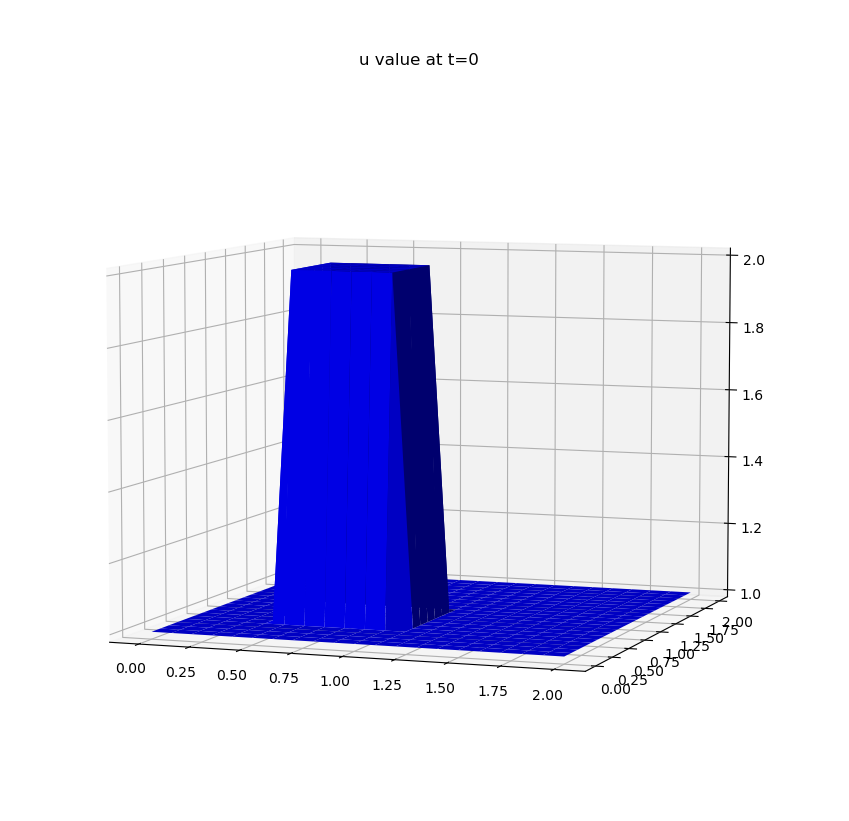
\includegraphics[scale=0.35]{images/u_initial.png}
		\caption{Initial value of U}
		\label{fig:01}
	\end{subfigure}
\begin{subfigure}{0.5\textwidth}
	\centering
	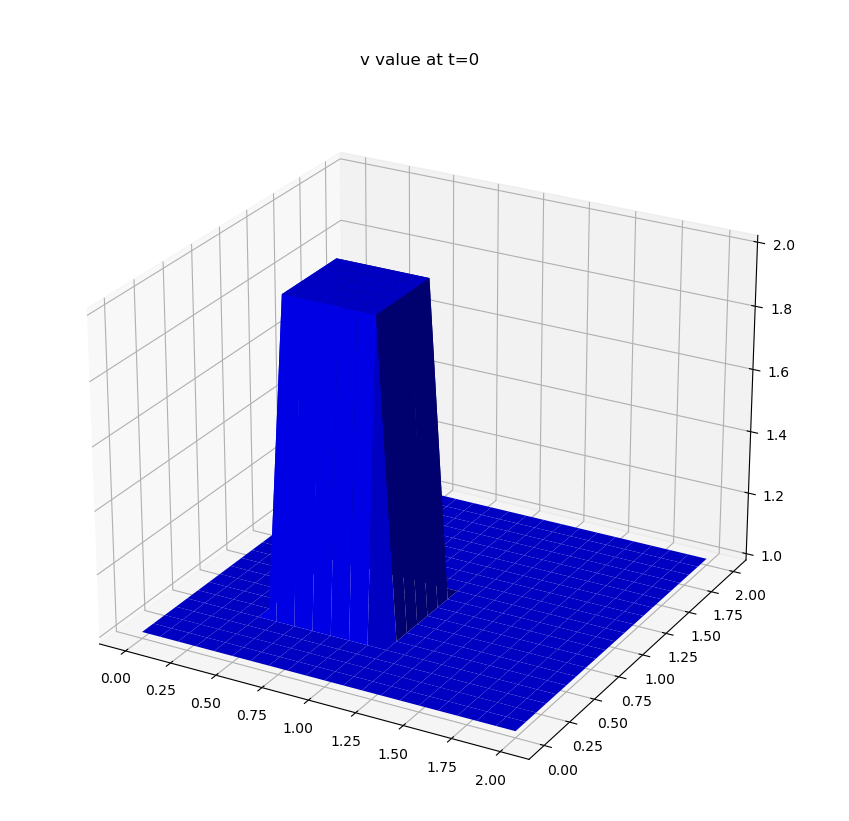
\includegraphics[scale=0.35]{images/v_initial.png}
	\caption{Initial value of V}
	\label{fig:02}
\end{subfigure}
\end{figure}
\begin{figure}[!h]
	\begin{subfigure}{0.5\textwidth}
		\centering
		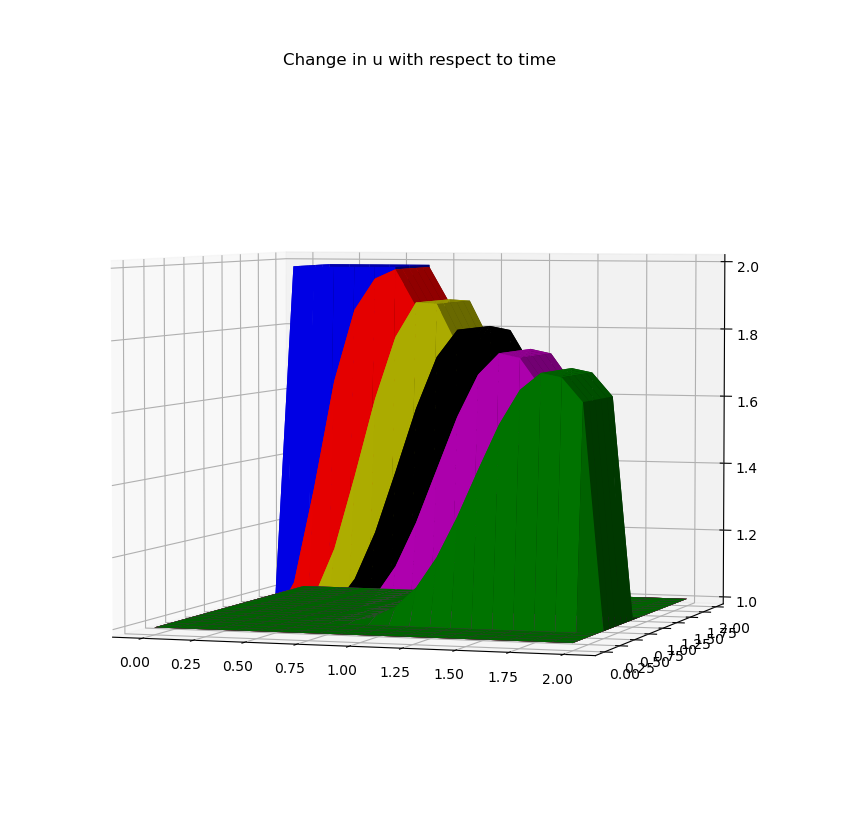
\includegraphics[scale=0.35]{images/u_c.png}
		\caption{Linear Convection of U at each 0.1 time steps}
		\label{fig:03}
	\end{subfigure}
	\begin{subfigure}{0.5\textwidth}
		\centering
		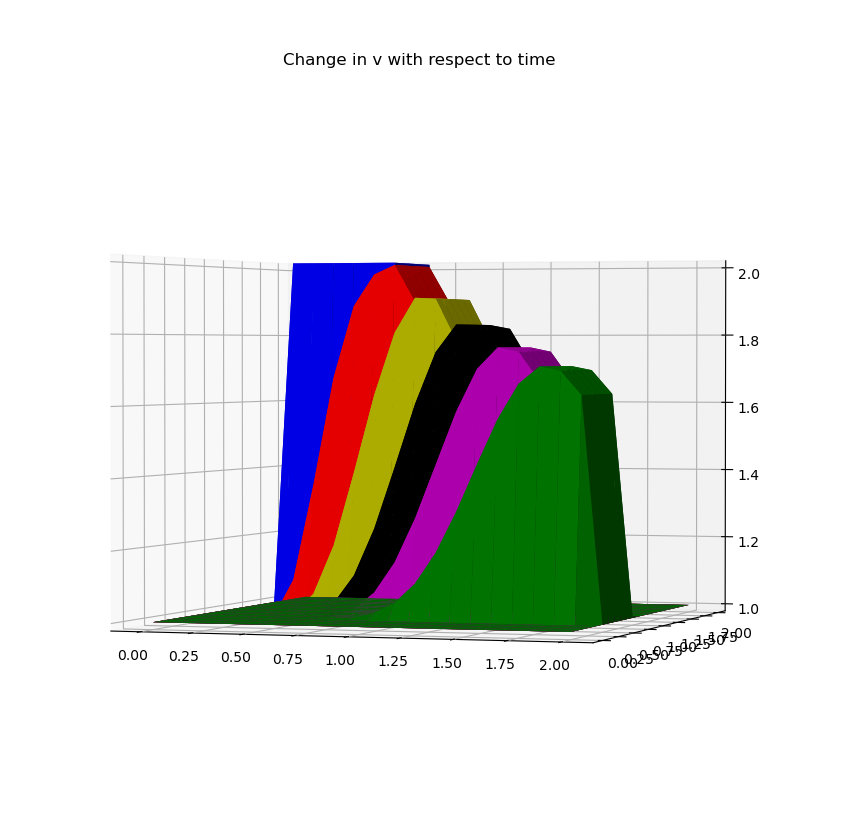
\includegraphics[scale=0.35]{images/v_c.png}
		\caption{Linear Convection of V at each 0.1 time steps}
		\label{fig:04}
	\end{subfigure}
\end{figure}
\begin{figure}[!h]
	\begin{subfigure}{0.5\textwidth}
		\centering
		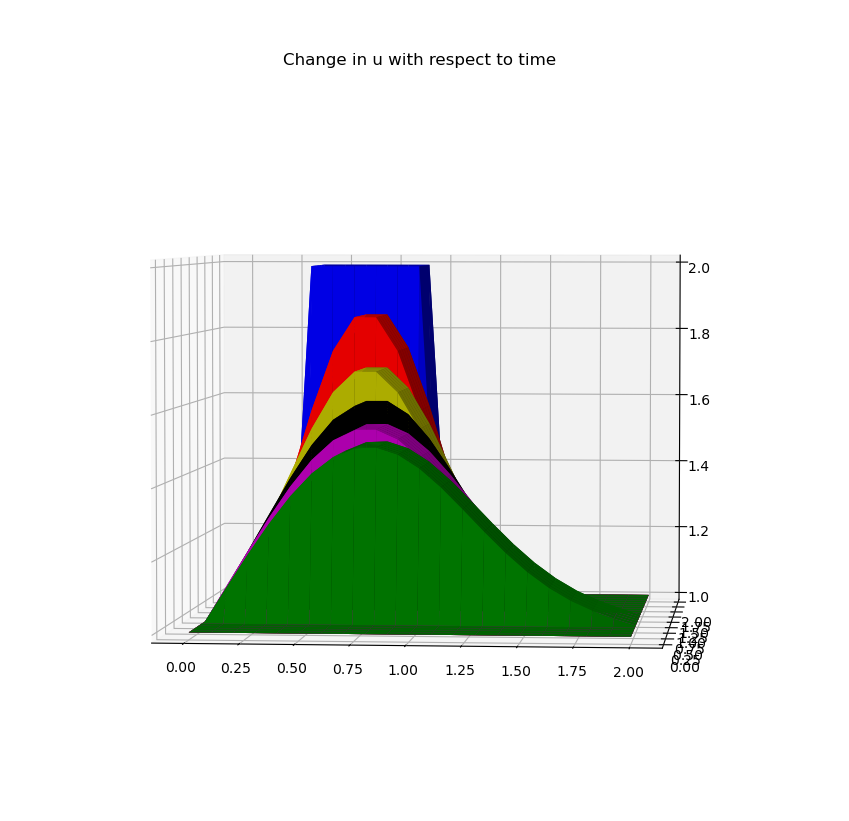
\includegraphics[scale=0.35]{images/u_d.png}
		\caption{Linear Diffusion of U at each 0.1 time steps}
		\label{fig:05}
	\end{subfigure}
	\begin{subfigure}{0.5\textwidth}
		\centering
		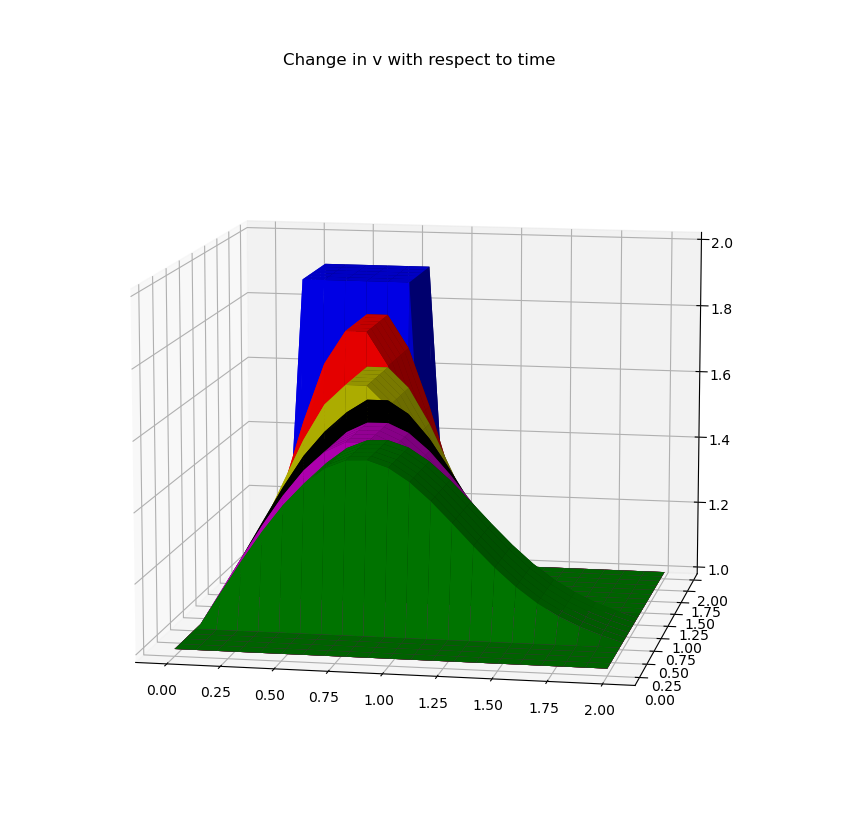
\includegraphics[scale=0.35]{images/v_d.png}
		\caption{Linear Diffusion of V at each 0.1 time steps}
		\label{fig:06}
	\end{subfigure}
\end{figure}

\pagebreak
 \begin{appendices}
      \section{Appendix - Python code for Linear Convection}\label{appendixA}


      \lstinputlisting[language=Python]{Code/2d_wave.py}

      \pagebreak

	\section{Appendix - Python code or Linear Diffusion}\label{appendixB}

	\lstinputlisting[language=Python]{Code/2d_diff.py}

	\pagebreak
\end{appendices}
\end{document}
